\documentclass[11pt]{article}
\usepackage[a4paper,margin=2.5cm]{geometry}
\usepackage{amsmath,amssymb}
\usepackage{booktabs}
\usepackage{array}
\usepackage{graphicx}

\newcommand{\Tsft}{T_{\rm SFT}}
\newcommand{\Tlim}{T_{\rm SFT}^{\rm lim}}
\newcommand{\Mc}{\mathcal{M}}

\title{Detection statistic $n_\sigma$ as a function of chirp mass and SFT duration\\
in the remapped $(t, f^{-8/3})$ search}
\date{}

\begin{document}
\maketitle

We derive the dependence of the detection statistic $n_\sigma$ on the chirp mass
$\Mc$ and on the SFT duration $\Tsft$, following the steps of
Ref.~[arXiv:2401.02314] and indicating where the present search differs from it.

\section{Definition of $n_\sigma$}

The Viterbi algorithm accumulates the normalised power of the pixels along the
recovered track. In the absence of a signal, the sum over $N_{\rm SFT}$ pixels has a
mean $\mu \propto N_{\rm SFT}$ and a standard deviation $\sigma \propto \sqrt{N_{\rm SFT}}$.
A signal increases the sum by its total optimal squared signal-to-noise ratio
$\rho^2_{\rm tot}$, so that
\begin{equation}
  n_\sigma = \frac{\rho^2_{\rm tot}}{\sigma} \propto \frac{\rho^2_{\rm tot}}{\sqrt{N_{\rm SFT}}} .
  \label{eq:nsigma}
\end{equation}
This is Eq.~(2.21) of Ref.~[arXiv:2401.02314]. The noise background measured in the
present search follows $\sigma \propto \Tsft^{-0.503}$, i.e.\ $\sigma \propto \sqrt{N_{\rm SFT}}$.

\section{Signal-to-noise ratio of the signal}

For an inspiral, $|\tilde h(f)|^2 \propto \Mc^{5/3} f^{-7/3}$, and therefore
\begin{equation}
  \rho^2_{\rm tot} \propto \Mc^{5/3} \int \frac{df}{f^{7/3} S_n(f)} ,
  \label{eq:rho}
\end{equation}
where the integral extends over the frequencies at which the Viterbi algorithm is
able to follow the signal. This step is identical to Ref.~[arXiv:2401.02314].

\section{Number of noise steps}

In Ref.~[arXiv:2401.02314] only the time during which the signal is present is
considered, $N_{\rm SFT} = T_{\rm CBC}/\Tsft$. In the present search, the Viterbi
algorithm runs over the whole data chunk, so that
$N_{\rm SFT} = T_{\rm obs}/\Tsft$ with $T_{\rm obs} = 32768$~s fixed. Since
$T_{\rm obs}$ depends neither on the chirp mass nor on $\Tsft$, it enters only as a
constant:
\begin{equation}
  n_\sigma \propto \sqrt{\frac{\Tsft}{T_{\rm obs}}}\; \Mc^{5/3} \int \frac{df}{f^{7/3} S_n(f)} .
  \label{eq:nsigma_tobs}
\end{equation}
In both cases the factor $\sqrt{\Tsft}$ appears: longer SFTs imply fewer noise steps.

\section{Frequency range over which the signal is tracked}

This is the key difference between the two approaches.

\paragraph{Linear frequency map (Ref.~[arXiv:2401.02314]).}
The signal is tracked as long as it remains within a single linear frequency bin
during one SFT, i.e.\ up to the frequency $f_\ast(\Tsft)$ defined by
$\dot f(f_\ast)\,\Tsft^2 = 1$; above it, the signal is lost:
\begin{equation}
  n_\sigma^{\rm lin} \propto \sqrt{\Tsft} \int_{f_0}^{f_\ast(\Tsft)} \frac{df}{f^{7/3} S_n(f)} .
  \label{eq:nsigma_lin}
\end{equation}
Two effects compete: increasing $\Tsft$ increases $\sqrt{\Tsft}$ but lowers
$f_\ast$, removing high frequencies from the integral. The optimum lies where both
effects balance, which yields Eq.~(14) of the paper.

\paragraph{Remapped map (present search).}
In the $(t, f^{-8/3})$ map the signal is a straight line with constant drift. The
Viterbi algorithm therefore follows it either over the \emph{whole} band or not at
all, depending on whether the signal moves by at most one remapped bin per step,
i.e.\ on whether $\Tsft \le \Tlim$. The integral no longer depends on $\Tsft$, and
only a cutoff remains:
\begin{equation}
  n_\sigma \propto \sqrt{\Tsft} \int_{f_0}^{f_1} \frac{df}{f^{7/3} S_n(f)}\;
  \Theta\!\left(\Tlim - \Tsft\right) .
  \label{eq:nsigma_remap}
\end{equation}

\section{Final expression}

Normalising to the maximum over $\Tsft$ at each chirp mass, as in Fig.~2 of
Ref.~[arXiv:2401.02314], the integral and all constant factors cancel:
\begin{equation}
  \frac{n_\sigma(\Mc, \Tsft)}{\max_{\Tsft} n_\sigma} =
  \begin{cases}
    \sqrt{\Tsft / \Tlim(\Mc)} , & \Tsft \le \Tlim(\Mc) , \\[4pt]
    0 , & \Tsft > \Tlim(\Mc) ,
  \end{cases}
  \label{eq:nsigma_norm}
\end{equation}
with
\begin{equation}
  \Tlim \simeq 17.7~{\rm s} \left(\frac{\Mc}{10^{-2}\,M_\odot}\right)^{-5/6}
  \qquad (f_0 = 61.1~{\rm Hz},\; f_1 = 126.8~{\rm Hz}) .
  \label{eq:tlim}
\end{equation}

\section{Validation with injections}

Equation~\eqref{eq:nsigma_norm} was tested with 75 injections into O3b data:
five chirp masses ($5.6\times10^{-4}$, $1.6\times10^{-3}$, $3.2\times10^{-3}$,
$1.8\times10^{-2}$ and $5.0\times10^{-2}\,M_\odot$), each at five distances ranging
from loud signals to the detection limit, and three random data chunks per point.
For each injection, $n_\sigma$ was computed for the 13 SFT durations of the search.
Since only these discrete values are available, the maximum is reached at
$T_{\rm ref}$, the largest $\Tsft$ of the grid not exceeding $\Tlim$, and the
prediction becomes $\sqrt{\Tsft/T_{\rm ref}}$.

\paragraph{Optimum.} For every detected signal the maximum of $n_\sigma$ is
reached at $T_{\rm ref}$, and $n_\sigma$ drops to the noise level for
$\Tsft > \Tlim$, as predicted.

\paragraph{Shape near the optimum.} The relevant range is $\Tsft$ close to
$\Tlim$, since the search always uses the largest available $\Tsft \le \Tlim$ and
consecutive values of the grid differ by a factor of 1.3--1.5. Within
$T_{\rm ref}/3 \le \Tsft \le T_{\rm ref}$ and for signals with
$\max n_\sigma \gtrsim 10$, the measured normalised $n_\sigma$ differs from
$\sqrt{\Tsft/T_{\rm ref}}$ by at most 0.13 (in absolute value of the normalised
quantity) and by less than 0.09 on average. Equation~\eqref{eq:nsigma_norm} is
therefore a very good approximation in the regime in which the search operates.

\paragraph{Shape far from the optimum.} For $\Tsft \ll \Tlim$ the measured
$n_\sigma$ falls below $\sqrt{\Tsft}$, increasingly so for weaker signals: with
short SFTs the signal-to-noise ratio per step, $\propto\sqrt{\Tsft}$, is low and
the Viterbi algorithm does not follow the signal in every step. These SFT
durations are never selected for the corresponding chirp masses, so this
deviation does not affect the choice of $\Tsft$.

\paragraph{Dense set of SFT durations.} To test the expression close to $\Tlim$,
we built the smallest set of SFT durations for which
Eq.~\eqref{eq:nsigma_norm} guarantees $n_\sigma \ge 0.95\,\max n_\sigma$ for every
chirp mass in $[2\times10^{-4}, 0.1]\,M_\odot$: 45 values from 2.6 to 422~s,
consecutive values differing by a factor $\simeq 1.11$. The noise background was
measured for every value, and three chirp masses were injected at five distances
each, with three data chunks per point. Now $T_{\rm ref}$ lies within 11\% of $\Tlim$
(Fig.~\ref{fig:dense}). For all detected signals the maximum is reached at
$T_{\rm ref}$, and $n_\sigma$ drops to the noise level above $\Tlim$. Within
$T_{\rm ref}/3 \le \Tsft \le T_{\rm ref}$:
\begin{itemize}
  \item for $\Mc = 5.0\times10^{-2}\,M_\odot$, the measured curves follow
    $\sqrt{\Tsft/T_{\rm ref}}$ within 0.09;
  \item for $\Mc = 3.2\times10^{-3}\,M_\odot$, within 0.17, with a mean deviation
    below 0.04;
  \item for $\Mc = 5.6\times10^{-4}\,M_\odot$, the measured $n_\sigma$ lies
    \emph{above} $\sqrt{\Tsft/T_{\rm ref}}$, by 0.10--0.15 on average: the gain
    flattens close to $\Tlim$.
\end{itemize}
Equation~\eqref{eq:nsigma_norm} is therefore accurate for heavy and intermediate
chirp masses, and a conservative lower bound for light ones. One step below
$T_{\rm ref}$ in the set, the measured normalised $n_\sigma$ is 0.93--0.99
(median 0.96), consistent within the scatter between data chunks with the
predicted 0.94--0.96.

\begin{figure}[h]
  \centering
  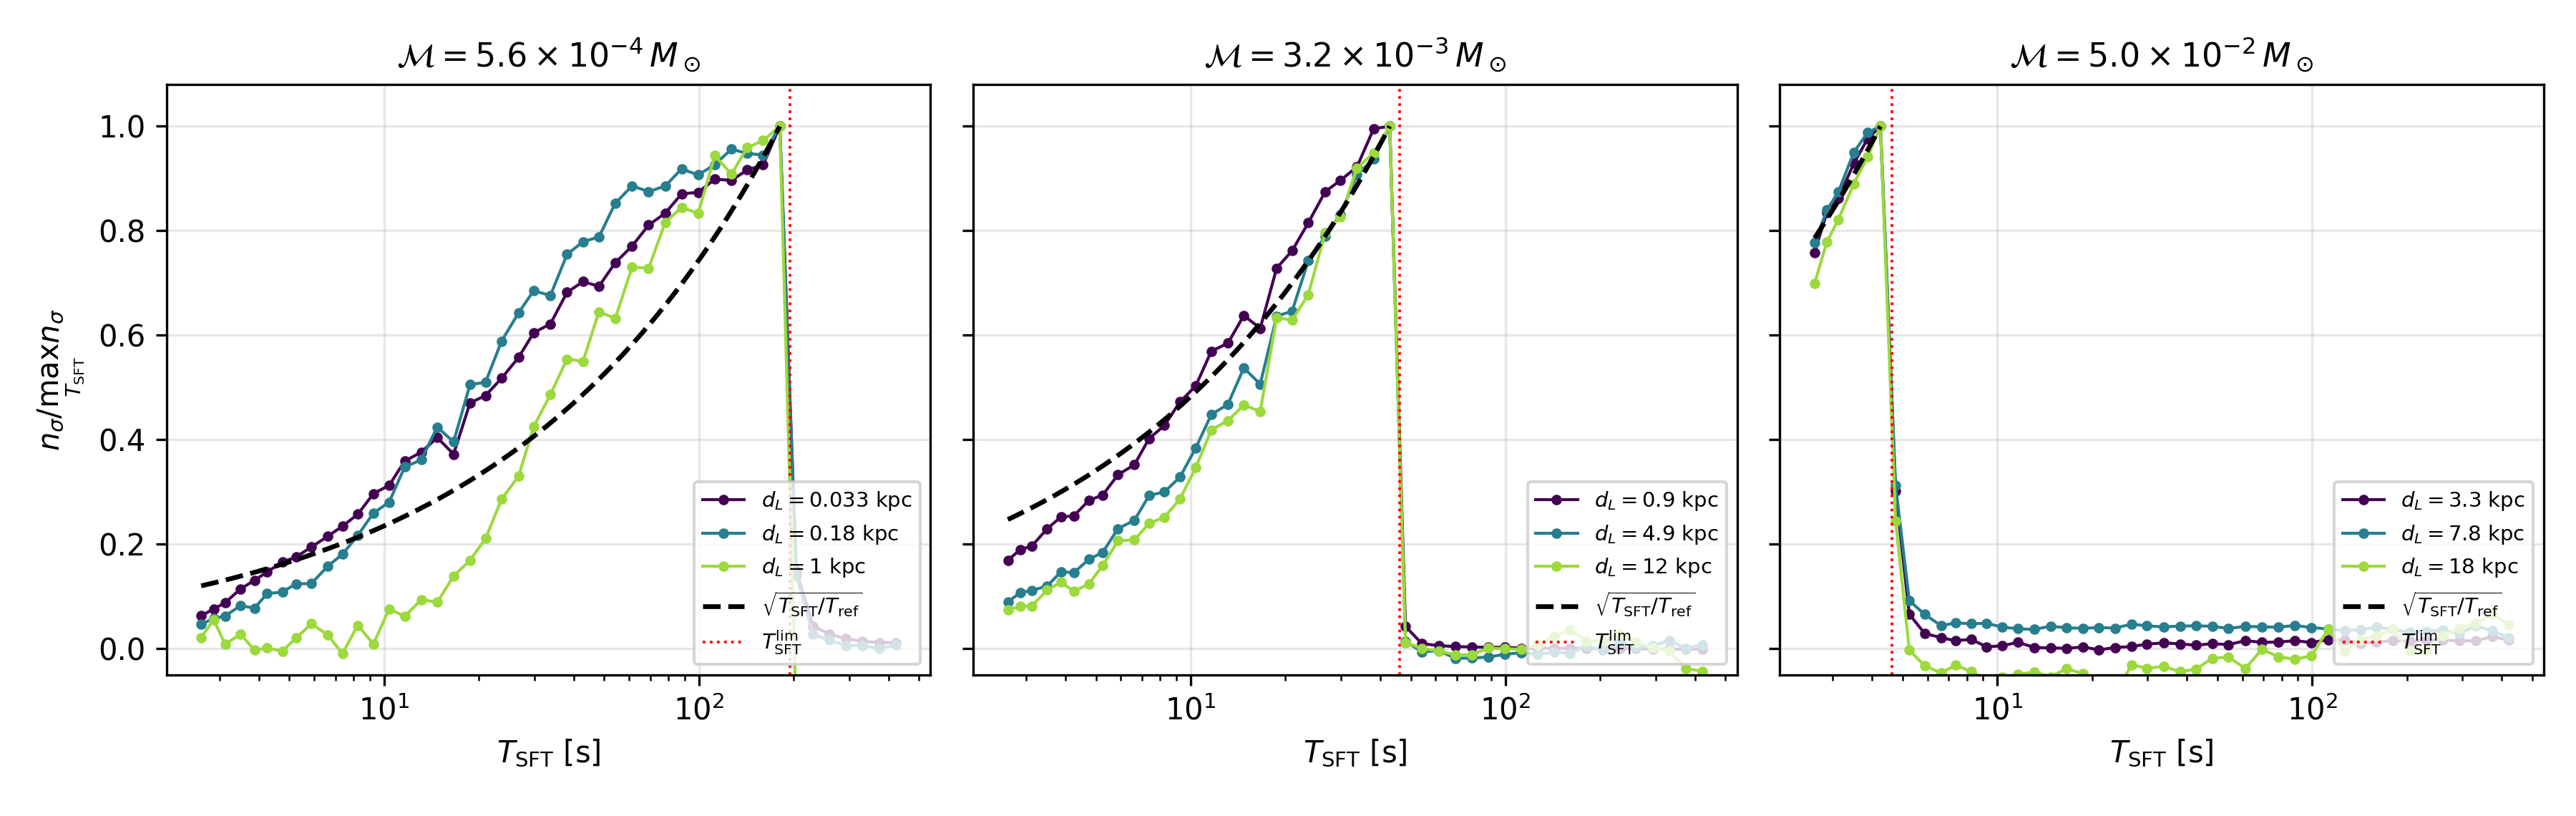
\includegraphics[width=\textwidth]{../../docs/figures/nsigma_vs_tsft_dense.png}
  \caption{Normalised $n_\sigma$ as a function of $\Tsft$ for the dense set of 45 SFT
    durations, for three chirp masses and several luminosity distances $d_L$
    (median over three data chunks; only detected signals are shown). The dashed
    line is $\sqrt{\Tsft/T_{\rm ref}}$, and the dotted line marks $\Tlim$.}
  \label{fig:dense}
\end{figure}

Table~\ref{tab:comparison} summarises the differences between both approaches.

\begin{table}[h]
  \centering
  \renewcommand{\arraystretch}{1.3}
  \begin{tabular}{>{\raggedright}p{0.2\textwidth} >{\raggedright}p{0.34\textwidth} >{\raggedright\arraybackslash}p{0.34\textwidth}}
    \toprule
     & Ref.~[arXiv:2401.02314] (linear frequency map) & Present search (remapped map) \\
    \midrule
    Noise steps & $T_{\rm CBC}/\Tsft$ & $T_{\rm obs}/\Tsft$ \\
    Tracking limit & $f_\ast(\Tsft)$: one linear bin per SFT & $\Tlim$: one remapped bin per step \\
    Effect of increasing $\Tsft$ & Gradual loss of high frequencies & No loss up to $\Tlim$, total loss beyond \\
    Optimum & Balance between $\sqrt{\Tsft}$ and the integral [Eq.~(14)] & Largest $\Tsft \le \Tlim$ \\
    Normalised $n_\sigma$ & Smooth around the optimum & $\sqrt{\Tsft/\Tlim}$ with a sharp cutoff \\
    \bottomrule
  \end{tabular}
  \caption{Comparison of the dependence of $n_\sigma$ on $\Tsft$ in
    Ref.~[arXiv:2401.02314] and in the present search.}
  \label{tab:comparison}
\end{table}

\end{document}
